\documentclass[11pt, oneside]{article}
\usepackage{geometry}
\geometry{a4paper}
\usepackage[parfill]{parskip}
\usepackage{graphicx}
\usepackage{amssymb}
\usepackage{amsmath}
\usepackage{MnSymbol}
\usepackage{hyperref} 

\def\undertilde#1{\mathord{\vtop{\ialign{##\crcr
$\hfil\displaystyle{#1}\hfil$\crcr\noalign{\kern1.5pt\nointerlineskip}
$\hfil\tilde{}\hfil$\crcr\noalign{\kern1.5pt}}}}}

\begin{document}

\begin{titlepage}
	\centering
	{\scshape\LARGE Evaluate Vanishing Point as Predictor for Steering Angle \par}
	\vspace{1cm}
	{\scshape\Large Oct 27, 2016\par}
	\vspace{2cm}
	{\Large\itshape Zeyi Wang\par}
	Department of Biostatistics\par
	\textsc{Johns Hopkins School of Public Health}

	\vfill

% Bottom of the page
%	{\large \today\par}
\end{titlepage}



\section*{Introduction}

The techniques of self-driving vehicles have been rapidly developed recently by using laser or video data and novel artificial intelligence algorithms. The Google Self-Driving Car Project 
\cite{google} relies on an advanced laser system and 3D imaging techniques. The comma.ai
\cite{comma.ai} 
uses mainly video data to mimic human drivers by 
training a conditional Recurrent Neural Network for transition model. 
One of the challenges is the computational efficiency needed for real-time reaction to the collected data including the complex data from space or vision sensors. 

This paper presents a simple robust method for vanishing point detection using video data and evaluates its role as a steering angle predictor using random forest algorithm. The method helps simplify the video processing and as well provides important reference for driving direction. A potentially more efficient self-driving model could be built in the future based on its prediction results. 

\section*{Data Sources}

The dataset we uses was published by comma.ai on its GitHub repository in July 2016. We downloaded it on September 17, 2016 using the get\_data.sh code shared by comma.ai. 

The dataset consists of 10 clips of videos at 20Hz and the 10 log files at 100Hz of measurements including speed, acceleration, steering angle, gps,  data collected by lidar, etc. 

\section*{Methods}

\subsection*{Exploratory analysis}

All the video files consist of frames of $320$ by $160$ RGB images and are stored as $n\times 3\times 320 \times 160$ four dimensional arrays. 

The log data is merged with respect to the time line of video files so that the merged video and log data will both be at 20Hz. 

\subsection*{Dynamic lane markings detection}

The lane markings are detected for the videos with the use of dynamic thresholds so that the detection could be robust against different lighting conditions. 

Each frame of the video of interest, which is a $320$ by $160$ RGB image, is converted into grayscale. It is then transformed by a Roberts cross operator, which is one of the common edge detectors. A $97\%$ quantile threshold is applied to the transformed image data to get the detected lane markings. The detected markings are stored in a $320$ by $160$ matrix of $\{0, 1\}$ values. 

We use Roberts cross operator mostly because it is computationally inexpensive and usually faster than other edge detectors. It is also because we do not need more accurate lane markings for the next step of getting vanishing point. 

The $97\%$ threshold is rather arbitrary for the similar consideration of computational efficiency and the tolerence for slightly lower accuracy. But we do prefer a dynamic quantile threshold that could vary as lightness changes rather than a static threshold. The benefit of such dynamic threshold should allow robust lane marking detection against the different lighting conditons. 

\begin{figure}[!ht]
  \centering
      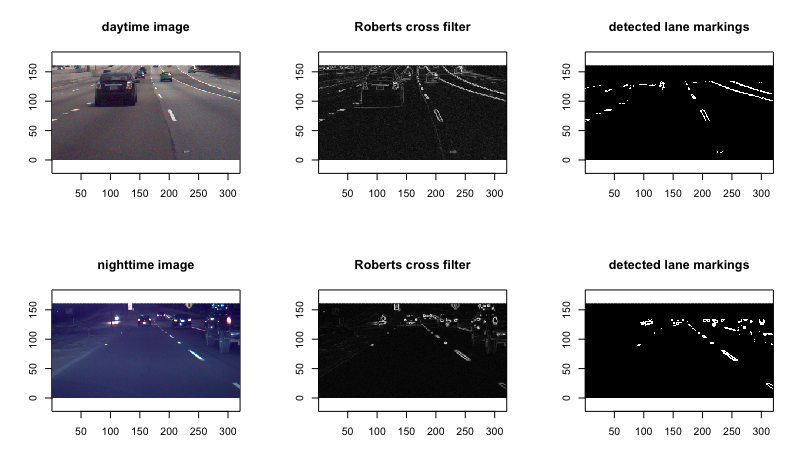
\includegraphics[width=0.9\textwidth]{Rplot1.png} 
  \caption{\textit{Dynamic 97\% quantile threshold} handles different lighting conditions}
\end{figure}


\subsection*{Vanishing points prediction}

A vanishing point in a picture is the intersection of a set of lines that are actually parallel in the real space. Our goal is to detect the vanishing point corresponding to the principal direction of the image, which we believe should unveil much information for an appropriate steering angle.

The first step is collecting line segments from the $\{0, 1\}$ valued lane marking matrix. Hough transformation, as one of the typical tools for line identification, is applied to the matrix. Such transformation will map all possible lines from the original matrix into entries of a new matrix. The value at each entry of the new matrix represents the "voting" information from the original image, that is, how many $1$-valued points in the original matrix intersect with the line corresponding to this specific entry. Lines with higher corresponding values in the new matrix, i.e. the Hough lines, are collected. 

The second step is predicting the vanishing points with the collected lines. For example, center of all the intersections of those lines could possibly be a solution. But further effort is required for more robust results. 

\subsection*{Improvements on robustness}

The Hough transformation and such searching process are relatively sensitive to noise. If some areas in the lane marking matrix is dense with more points, the collected Hough lines will mostly be related with such areas, and the information outside such areas will be ignored. In which case, Hough lines will be close to each other and provide limited information so that we can hardly infer principal direction from them.  The unstable predicted points might as well lie out of image, move dramatically or not even exist. We then propose an improved robust version of the vanishing point prediction.

First of all, the upper 25 rows of pixels are re-valued as $0$ because they are usually related to the sky and provide no information for direction. 

Second, we partition the left lane marking matrix evenly into the left part and the right part and then search Hough lines seperately. Even if points are dense in one side of the matrix due to some noise, we can still balance it with the information from the other part so that we are able to find a prediction closer to the real principal direction. The prediction will be given using the intersections of Hough lines from both parts. 

Third, we only collect the intersection of a pair of Hough lines if the difference of their slopes is greater than $0.2$. If such process finds no eligible intersection, we let vanishing point locate at the center. 

Fourth, ideally the prediction of vanishing point sould be somehow stable because in reality we drive following the road which will not change its direction dramatically or totally at random. 

Kalman filter is one of such techniques that allows us to better estimate the more stable true process with unstable and uncertain observations. It is especially favorable for target tracking with its recursive feature so that the new observations could be processed as they arrive. 

We applied the Kalman filter to the series of crude prediction of vanishing points in a real time manner. Therefore the stablized prediction filtered by all the previous points will be our best guess for the vanishing point. 

\begin{figure}[!ht]
  \centering
      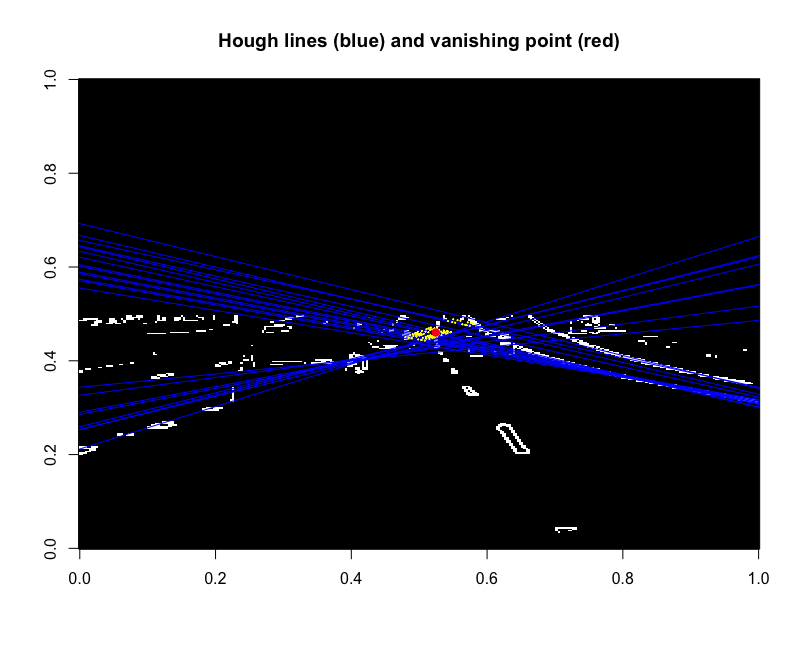
\includegraphics[width=0.9\textwidth]{Rplot2.png} 
  \caption{\textit{Robust prediction of vanishing point}}
\end{figure}

Note here that: 1. The upper 25 rows of pixels are discarded; 2. Hough lines are collected from left and right parts seperately; 3. only eligible intersections (small yellow dots) are counted for the final prediction;


\subsection*{Evaluate vanishing point as a predictor for steering angle}

A steering angle prediction model is fitted on the training set using the vanishing point results above. 

Suppose the training set includes $T$ time points of video and log data. At each time point $t \in \{1, \cdots, T\}$, we have predicted vanishing point $V(t) = (V_x(t), V_y(t))$. We collect speed $S(t)$ and steering angle $A(t)$. We assume that there exists a prediction model $f$ for the appropriate steering angle $A$:
$$
f(V_x(t-1), V_y(t-1), S(t-1)) = A(t).
$$
We expect that the model is approximately estimable in reality and could be fitted with default random forest algorithm. 

The accuracy of prediction is then calculated on the test set. The importance of predictors are also reported. 

The reason we use random forest algorithm is that it handles overfitting and also provides information on importance of predictors. 

\section*{Results}

From files "./camera/2016-06-08--11-46-01.h5" and "./log/2016-06-08--11-46-01.h5", we clipped a training set of $100$ seconds (tiem points 11000-13000) and a test set of $70$ seconds (time points 13001-14400). Both are of daytime highway driving records under normal weather condition. 

Vanishing points $V(t) = (V_x(t), V_y(t))$ are estimated for all time points of interest. Speed $S(t)$ and steering angle $A(t)$ are also collected. 


On the training set, the prediction model for steering angle is fitted, reporting root mean square error (RMSE) for steering angle prediction of 5.05 on the training set and 2.11 on the test set. The mean and standard error of the original steering angle records (in a format of mean(sd)) are -0.05(5.6) on the training set and -0.24(2.97) on the testing set. 

The reported importance measurement (total decrease in node impurity) for speed $S$ and two components $V_x$ and $V_y$ of the vanishing points are 0, 21486.95 and 5199.43, suggesting that vanishing point is the most important predictor for this model. 

The result is also visualized using the speed, the steering angle record (in blue), the predicted steering angle (in green). The formula and mechanical parameters for visualization are cited from the code shared by comma.ai \cite{github}. Links for our visualized results are:

\href{https://youtu.be/E4DUmLJFs_c}{test}
\begin{verbatim}
https://youtu.be/E4DUmLJFs_c
\end{verbatim}

\href{https://youtu.be/p2RmdN7Chl0}{train}
\begin{verbatim}
https://youtu.be/p2RmdN7Chl0
\end{verbatim}
. 

\begin{figure}[!ht]
  \centering
      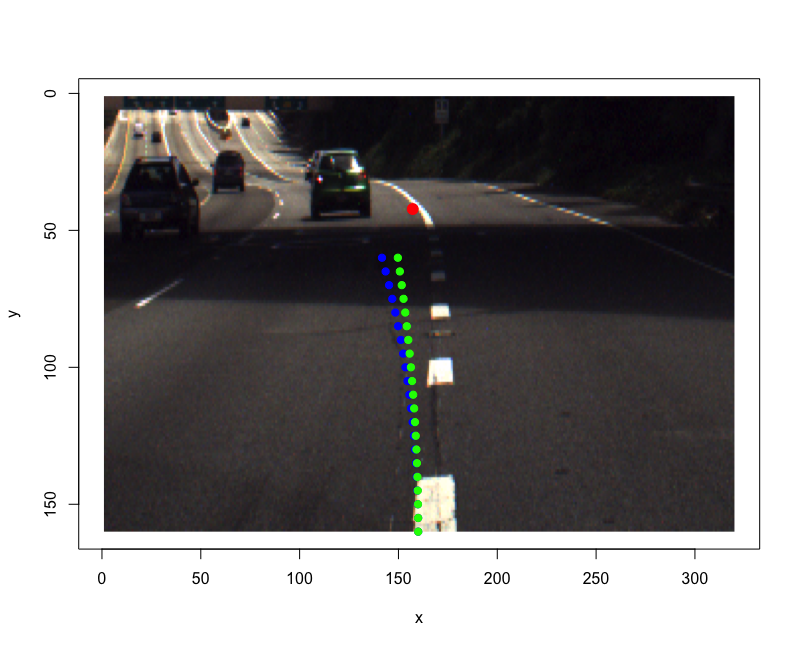
\includegraphics[width=0.9\textwidth]{Rplot3.png} 
  \caption{\textit{Visualization} of vanishing point (red), recorded direction (green) and predicted direction (blue)}
\end{figure}


\section*{Discussions}

\subsection*{Limitation of video data}

Although comma.ai claims that a well designed deep learning algorithm will be able to completely mimic human driving -- using only image data, we argue that it is actually unrealistic. There are at least two more features that human can take advantage of but a camera cannot: 1. moving parallax allows human to estimate distance by slightly moving their heads since the closer objects moving faster on the retina; 2. human actually have stereo vision from two eyes which is benefitial for distance estimation. Therefore using solely video data -- no matter how advanced the algorithm is -- must have a limit in accuracy of mimicing human drivers whereas an ultimate self-driving car has very little tolerance for error in many circumstances. 

Instead of spending all effort in image processing, we simplify the process so that the spare computational power could be used for other elements of the driving model. 

\subsection*{Role of current model and its limitations}

The goal of this model is not becoming a fully self-driving car on its own, but to provide an inexpensive yet somehow accurate predictor for steering angle when following traffic which could be an important element in the integrated self-driving system. 

The current model only works for the purpose of following traffic. If a request of turns or lane switching is received from GPS, the vehicle should turn down the current model and prepare for the change of driving route. 

Collision avoidance system using 3D lidar is needed, which requires advanced object tracking algorithm for 3D images. 

More complete system for specific traffic signal detection is needed. The system should accurately recognize different types of lanes, traffic signs including stop sign, traffic light, speed limit, etc. 

\subsection*{Potentials}

Transforming the road image to bird's eye view might help improve the accuracy and robustness of vanishing point prediction. 

A stabler tracking algorithm of lane markings could be built using particle filter but it might compromise in computational efficiency. 


A possible blueprint for an integrated self-driving system could be built by:\\
1. A tool for following traffic (current model); \\
2. An immediate reponse system processing emergent information such as important traffic signs or lanes detected, route instructions received from gps, or signals received from a collision advoidance system. \\
3. An Artifitial Intelligence system for more arbitrary decisions such as optional lane changes and acceleration. 





\bibliographystyle{plain}
\bibliography{final}

\end{document}  